
% 4 paragraph intro

To communicate successfully, speakers and listeners must share a common system of semantic meaning in the language they are using. 
These meanings are \emph{social conventions} in the sense that they are arbitrary to some degree, but sustained by stable expectations that each person holds about others in their community \cite{lewis_convention:_1969,bicchieri_grammar_2006, hawkins2019emergence}.
Importantly, these expectations extend to complete strangers.
An English speaker may order a ``cup of coffee'' at any café in the United States and expect to receive (roughly) the same kind of drink.

At the same time, meaning can be remarkably flexible and \emph{partner-specific}.
The same words may be interpreted differently by different listeners. 
Interactions between friends and colleagues are filled with proper names, technical jargon, slang, shorthand, and inside jokes, many of which are unintelligible to outside observers.
Furthermore, words easily take on new \emph{ad hoc} senses over the course of a conversation \cite{clark_using_1996}.

The tension between these two basic observations has posed a challenging and persistent puzzle for theories of convention.
Influential computational accounts explaining how social conventions emerge in populations \cite<e.g.>{skyrms2010signals,steels2011modeling,barr_establishing_2004,young_evolution_2015} typically do not allow for partner-specific meaning at all.
These accounts examine groups of interacting agents who update their representation of language after each interaction.
While the specific update rules range from simple associative mechanisms \cite<e.g.>{steels_self-organizing_1995} or heuristics \cite<e.g>{Young96_EconomicsOfConvention} to more sophisticated deep reinforcement learning algorithms \cite{tieleman2019shaping,graesser2019emergent,mordatch2017emergence}, all of these accounts assume that agents update a single, monolithic representation of language to be used with every partner, and that agents do not (knowingly) interact repeatedly with the same partner.

Conversely, accounts emphasizing rapid alignment \cite{pickering2004toward} and partner-specific common ground \cite{ClarkWilkesGibbs86_ReferringCollaborative} across extended interactions with the same partner typically do not specify mechanisms by which community-wide conventions may arise over longer timescales.
The philosopher Donald Davidson articulated one of the most radical of these accounts.
According to \citeA{davidson1984communication,davidson_nice_1986,davidson1994social}, it is exclusively the ability to coordinate on \emph{partner-specific} meanings that is ultimately responsible for successful communication.
This line of argument led \citeA{davidson_nice_1986} to memorably conclude that ``there is no such thing as a language'' (p.~265), and to abandon appeals to convention altogether \cite<see also>[for discussion]{heck_idiolect,lepore2007reality,hacking1986nice,dummett1994}.%\footnote{ In Davidson's terminology, the system of meanings given by from convention is called the agent's \emph{prior} theory, while the ad hoc systems they form with their partner on the fly are called their \emph{passing} theories. We maintain this distinction, but instead call these \emph{global} conventions and \emph{local} or \emph{ad hoc} conventions, respectively, to emphasize their commonality.}.

In this paper, we propose a theory of coordination and convention that aims to reconcile the emergence of community-level conventions with partner-specific common ground in a unified cognitive model.
This theory is motivated by the computational problems facing individual agents who must communicate with one another in a variable and non-stationary world. 
We suggest that three core cognitive capacities are needed for an agent to solve this problem, which are naturally formalized in a hierarchical Bayesian model:
\begin{description}
\item[C1:] the ability to maintain \textbf{uncertainty} about what words will mean to different partners,
\item[C2:] flexible  \textbf{online learning} to coordinate on partner-specific meanings, and
\item[C3:] inductive \textbf{generalization} to abstract away stable expectations to new partners.
\end{description}
Indeed, one of our central theoretical aims is to ground the problem of convention --- a fundamentally interactive, social phenomenon --- in the same domain-general cognitive mechanisms supporting learning in other domains where abstract, shared properties need to be inferred along with idiosyncratic particulars of instances \cite{berniker2008estimating,GoodmanUllmanTenenbaum11_TheoryOfCausality,tenenbaum_how_2011,kleinschmidt2015robust}.

%\begin{enumerate}
%\item \textbf{Lexical uncertainty:} When we first encounter a new communication partner in a new context, we call upon some representation about what we think different signals mean to them. This representation of meaning must be sensitive to the overall statistics of the population: more people are familiar with the use of \emph{dog} to refer to the beloved pet than \emph{sclerotic aorta} to refer to the potentially dangerous health condition. It must also be sensitive to the immediate context of the interaction: a cardiologist should have different expectations about a novel colleague than a novel patient.
%\item \textbf{Rapid adaptation:} Within a few minutes of conversation, we can considerably strengthen our expectations about our partner's lexicon based on earlier utterances and feedback, and adjust our own usage accordingly. For example, even if we are not initially familiar with the term \emph{sclerotic aorta}, a few minutes spent discussing the condition in simpler terms should make us more confident using the term with that partner in the future. This social learning mechanism must allow for signal \emph{reduction} -- simpler, more efficient ways of referring to the same thing over time -- and \emph{path-dependence}: early reinforcement of certain meanings increases their later usage, however arbitrary or provisional they began. 
%\item \textbf{Generalization:} When we encounter the same partner in a new context, we should expect some `stickiness' from previous learning. Language does not reset at context boundaries. In addition, the lexical model we've learned within a conversation should be largely \emph{partner-specific}. Just because we now expect Partner A to be familiar with a \emph{sclerotic aorta} shouldn't radically change our expectations about Partner B. Over enough interactions with different language users, however, our initial representations should be able to shift to take these data into account. To generalize appropriately, we must be able to correctly attribute whether a usage is idiosyncratic to a particular speaker, or a global convention we should expect to hold across the whole community.
%\end{enumerate}

Our argument is structured around a series of three key phenomena in the empirical literature that have proved evasive for previous theoretical accounts of convention and coordination: 
\begin{description}
\item[P1:] the convergence to increasingly \textbf{efficient} referring expressions over repeated interactions with a single partner,
\item[P2:] the influence of \textbf{partner-specificity} as conventions gradually generalize to new partners, and
\item[P3:] the influence of \textbf{communicative context} on which terms eventually become conventionalized 
\end{description}

We begin by introducing the \emph{repeated reference game} paradigm at the center of this literature and reviewing the empirical evidence supporting each of these phenomena.
We then introduce our hierarchical Bayesian model in detail and highlight several qualitative properties that emerge from our formulation.
The remainder of the paper proceeds through each of these phenomena (\textbf{P1}-\textbf{P3}) in turn. 
For each phenomenon, we use computational simulations to evaluate our model's explanations on existing data, and introduce data from new behavioral experiments to test novel predictions when existing data does not suffice.
Finally, we close by discussing several broader consequences of the theory.

\subsection{Three lessons about convention formation from repeated reference games}

A core function of language is \emph{reference}: using words to convey the identity of an entity in the environment. 
Loosely building on \citeA{wittgenstein2009philosophical}, empirical studies of coordination and convention in communication have predominantly focused on the subset of language use captured by simple ``reference games.'' 
In a reference game task, participants are assigned to speaker and listener roles and shown a context  of possible referential targets (e.g. images).
On each trial, the speaker is asked to produce a referring expression --- typically a noun phrase --- that will allow the listener to select the intended target object from among the other objects in the context.
Critically, a \emph{repeated reference game} asks them to refer to the same targets multiple times as they build up a shared history of interaction, or \emph{common ground,} with their partner (see Table \ref{table:parameters} in Appendix for a review of the different axes along which the design varies).

Unlike typical studies of referring expression generation \cite{van_deemter_computational_2016,degen2020redundancy,dale1995computational}, studies of coordination and convention tend to use novel, ambiguous stimuli that participants do not already have strong conventions for.
And unlike agent-based simulations of convention formation on large networks \cite{steels2011modeling,barr_establishing_2004,centola_spontaneous_2015}, which typically match agents with a new partner for each trial, repeated reference games ensure that participants maintain the same partner throughout an extended interaction.
This design allows us to observe how the speaker's referring expressions for the same objects change as a function of interaction with that particular partner.
We highlight three findings of particular theoretical significance in this literature.

\paragraph{Conventions rapidly increase in efficiency (\textbf{P1})}

The most well-known phenomenon observed in repeated reference games is a dramatic reduction in message length over multiple rounds \cite{krauss_changes_1964, ClarkWilkesGibbs86_ReferringCollaborative, hawkins2020characterizing}. 
The first time participants refer to a figure, they tend to use a lengthy, detailed description (``the upside-down martini glass in a wire stand'') but with a small number of repetitions --- between 3 and 6, depending on the pair of participants --- the description may be cut down to the limit of just one or two words (``martini''). 
These final messages are as short or shorter than the messages participants choose to allow \emph{themselves} to choose the target in the future  \cite{FussellKrauss89_IntendedAudienceCommonGround} and are often incomprehensible to overhearers who were not present for the initial messages \cite{SchoberClark89_Overhearers}.
These observations set up our first puzzle of \emph{ad hoc} convention formation in dyads.
How does a word or short phrase that would have been ineffective for communicating under the global conventions of a language take on local meaning over mere minutes of interaction? 

\begin{figure}[t!]
\centering
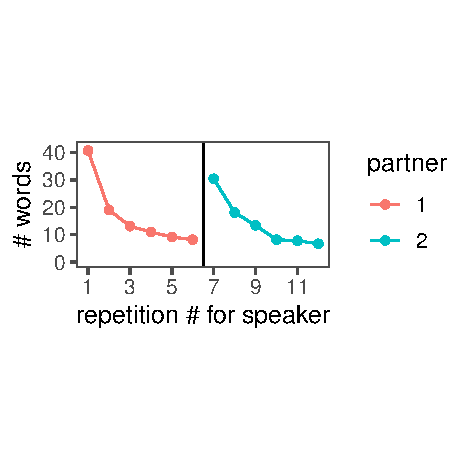
\includegraphics[scale=1.2]{./figures/clark92}
\vspace{1em}
\caption{\textit{Classic phenomena in repeated reference games.} Across multiple repetitions of the same referent with the same partner, speakers converge to increasingly efficient utterances (reps.~1-6). When the listener is  replaced by a new, naive partner, speakers display a key signature of partner-specificity, reverting to longer utterances before converging again with their new partner (reps.~7-12). Error rates were reported to be uniformly low ($\sim 2.3\%$) throughout the experiment. Reproduced from Table 3 in \protect\citeA{wilkes-gibbs_coordinating_1992}.}
\label{fig:clark92}
\end{figure}

\paragraph{Conventions may be partner-specific  (\textbf{P2})}

Because meaning is grounded in the evolving common ground shared with each partner, \emph{ad hoc} conventions established over a history of interaction with one partner are not necessarily transferred to other partners \cite{metzing_when_2003,weber_cultural_2003,horton_revisiting_2016}. 
For example, \citeA{wilkes-gibbs_coordinating_1992} paired participants for a standard repeated reference game, but after six rounds, one partner was asked to leave the room and replaced by a naive partner. 
Without partner-specific representations, we would expect speakers to continue using the short labels they had converged on with their first partner; instead, speakers reverted to the longer utterances they had initially used and coordinated on new \emph{ad hoc} conventions with their new partner (see Fig. \ref{fig:clark92}).

These effects raise our second puzzle: how do population-level conventions form in the presence of such strong partner-specificity?
When are agents justified in transferring an \emph{ad hoc} convention formed with one partner to a new, unseen partner? 
One important empirical clue was provided by \citeA{fay_interactive_2010}, who examined the emergence of conventions in a lab experiment where communities of eight people played a repeated (non-linguistic) Pictionary game with each partner in turn, for a series of seven repeated reference games in a row. 
Strikingly, while participants reverted to their initial messages with the first few partners, consistent with partner-specificity, the initial messages they sent to subsequent partners gradually converged closer to the final \emph{ad hoc} messages they used with previous partners, indicating a slow gradient of generalization mixed with partner-specificity.
While intriguing, this work was limited by an extremely small sample size ($N = 4$ groups) and technical challenges facing the measurement of conventions in the graphical modality \cite<see>{hawkins2019disentangling}.
We revisit this effect using a larger data set based on naturalistic linguistic communication.

\paragraph{Conventions are influenced by communicative context (\textbf{P3})}

Finally, while a degree of arbitrariness is central to conventionality -- there must exist more than one solution that would work equally well -- this does not necessarily imply that all possible conventions for a meaning are equally likely in practice, or even that all meanings are equally likely to become conventionalized in the first place \cite{HawkinsGoldstone16_SocialConventions}.
Functional accounts of language have frequently observed that lexical systems are well-calibrated to the statistics of the communicative environment \cite{gibson2019efficiency}.
This Optimal Semantic Expressivity  hypothesis \cite<OSE;>{frankblogpost}  has accounted well for the lexical distributions found in natural languages across semantic domains like color words and kinship categories \cite{KempRegier12_KinshipCategories,regier201511,gibson2017color,kemp2018semantic}.
For example, languages in warm regions ought to be more likely to collapse the distinction between ice and snow into a single word, simply because there are fewer occasions that require distinguishing between the two \cite{regier2016languages}. 

Such long-term, diachronic context-sensitivity has not yet been grounded in a cognitive and mechanistic account of the immediate, synchronic processes unfolding in the minds of individual agents in dyadic interaction.
Lab studies using repeated reference games have provided a more tractable way to examine the distribution of conventions that emerge when communicating with artificial languages \cite{WintersKirbySmith14_LanguagesAdapt, KirbyTamarizCornishSmith15_CompressionCommunication} and the efficient \emph{ad hoc} labels that dyads converge to when using natural language \cite{hawkins2020characterizing}.
However, it has remained challenging to directly evaluate cognitive models using these tasks.
While there is abundant empirical evidence for context-sensitivity in the \emph{outcomes} of convention formation processes, our third puzzle concerns which cognitive mechanisms are necessary or sufficient to give rise to such outcomes.


